\part{Techniques}
\chapter{Schur Complement and LU Decomposition}
\section{Preliminaries}
Usually, $|\A\B| \ne |\B\A|$. For example
\ex{
    \begin{align*}
        \begin{vmatrix}\left[\begin{matrix}1 ~~ 1\end{matrix}\right] \left[\begin{matrix}0 \\ 1\end{matrix}\right]\end{vmatrix} = \begin{vmatrix}1\end{vmatrix} = 1
    \end{align*}

    \begin{align*}
        \begin{vmatrix}\left[\begin{matrix}0 \\ 1\end{matrix}\right] \left[\begin{matrix}1 ~~ 1\end{matrix}\right]\end{vmatrix} = \begin{vmatrix}\left[\begin{matrix}0 ~~ 0 \\ 1 ~~ 1\end{matrix}\right]\end{vmatrix} = 0
    \end{align*}
}

However, the {\bf{Sylvester's Determinant Theorem}} says, as long as $\A\B$ and $\B\A$ are both square matrices,
\begin{align}
    \begin{vmatrix}\I+\A\B\end{vmatrix} = \begin{vmatrix}\I+\B\A\end{vmatrix}
\end{align}

It is also not true in general that
\begin{align*}
    \begin{vmatrix}\left[\begin{matrix}\A ~~ \B \\ \C ~~  \D\end{matrix}\right]\end{vmatrix} = \begin{vmatrix}\A\D-\B\C\end{vmatrix}
\end{align*}
unless $\C$ and $\D$ are commutable, i.e., $\C\D = \D\C$. The general formula for block determinant is
\begin{align}
    \begin{vmatrix}\left[\begin{matrix}\A ~~ \B \\ \C ~~  \D\end{matrix}\right]\end{vmatrix} = \begin{vmatrix}\A\end{vmatrix}\begin{vmatrix}\D - \C\A^{-1}\B\end{vmatrix}
\end{align}
which is based on Schur complement.

\section{Schur Complement and LU Decomposition}
Suppose we have a homogeneous linear system
\begin{align}
	\left[\begin{matrix}\A & \B \\ \C & \D \end{matrix}\right] \left(\begin{matrix} \x \\ \y \end{matrix}\right) = \left(\begin{matrix} \mathbf{0} \\ \mathbf{0} \end{matrix}\right)
\end{align}
To solve for $\y$, if $\A$ is nonsingular, we may multiply the first row by $-\C\A^{-1}$ and add to the second, and obtain
\begin{align}\label{eq:shurA}
	\left[\begin{matrix}\I & \mathbf{0} \\ -\C\A^{-1} & \I \end{matrix}\right] \left[\begin{matrix}\A & \B \\ \C & \D \end{matrix}\right] = \left[\begin{matrix}\A & \B \\ \mathbf{0} & \D-\C\A^{-1}\B \end{matrix}\right]	
\end{align}

\deff{
Suppose $\M$ is a square matrix $$\M = \left[\begin{matrix}\A & \B \\ \C & \D \end{matrix}\right]$$ and $\A$ nonsingular.
We denote \footnote{It is easy to remember if you multiply the submatrices clockwise.}
\begin{align}
	\M/\A = \D-\C\A^{-1}\B
\end{align}
and call it {\em{the Schur complement of $\A$ in $\M$}}, or {\em{the Schur complement of $\M$ relative to $\A$}}.

\rmk{
A very useful identity can be revealed from equation \ref{eq:shurA} \marginnote{\dbend}
\begin{align}
	\M = \left[\begin{matrix}\A & \B \\ \C & \D \end{matrix}\right] = \left[\begin{matrix}\I & \mathbf{0} \\ \C\A^{-1} & \I \end{matrix}\right] \left[\begin{matrix}\A & \mathbf{0} \\ \mathbf{0} & \D-\C\A^{-1}\B \end{matrix}\right] \left[\begin{matrix}\I & \A^{-1}\B \\ \mathbf{0} & \I \end{matrix}\right]
\end{align}
}which gives us the following identities
\thm{
\begin{align}
	det(\M) &= det(\M/\A) \cdot det(\A)\\
	rank(\M) &= rank(\M/\A) + rank(\A)
\end{align}
}
\rmk{
For a non-homogeneous system of linear equations $$\left[\begin{matrix} \A & \B \\ \C & \D \end{matrix}\right] \left(\begin{matrix} \x \\ \y \end{matrix}\right) = \left(\begin{matrix} \u \\ \v \end{matrix}\right)$$ We may use Schur complements to write the solution as
\begin{align}
	\x = (\M/\D)^{-1}(\u-\B\D^{-1}\v)\\
	\y = (\M/\A)^{-1}(\v-\C\A^{-1}\u)
\end{align}
}
\thm{
	If $\M$ is a positive-definite symmetric matrix, then so is the Schur complement of $\D$ in $\M$.
}


\chapter{The $\A\x=\b$ Problem}
\section{Solving a Linear System of Equations}
\thm{
	If $A = \left[\begin{matrix}a & b\\ c & d\end{matrix}\right]$, then $A$ is invertible if $ad-bc\ne 0$, in which case $$A^{-1} = \frac{1}{ad-bc} \left[\begin{matrix}d & -b\\ -c & a\end{matrix}\right]$$
}
\begin{rmk}
	Three ways to solve a system of linear equations: by elimination, by determinants {\color{red}{(Cramer's Rule???)}}, or by matrix decomposition.
\end{rmk}

\begin{rmk}
	We prefer to use matrix decomposition to solve a linear system because
	\begin{enumerate}
		\item It takes $\mathcal{O}(n^3)$ to factorize, but once done it can be used to solve systems with different $\b$ (right hand side).
		\item It is numerically more stable than computing $\A^{-1}\b$.
		\item For a sparse matrix, the inverse may be dense and may hard to store in memory. Decomposition can overcome this problem.
	\end{enumerate}
\end{rmk}

\begin{rmk}
	The computation of elimination is $\mathcal{O}(n^3)$, but can be (non-trivially) reduced to $\mathcal{O}(n^{\log_27})$.
\end{rmk}

\section{The Vector Spaces of a Matrix}
\begin{rmk}
	$Ax$ is a combination of the {\em{columns}} of $A$. $b^TA$ is a combination of the {\em{rows}} of $A$. Row picture can be seen as interchapter of (hyper-)planes. Column picture can be seen as combination of columns.
\end{rmk}

\begin{rmk}
	There are three different ways to look at matrix multiplication:
	\begin{enumerate}
		\item Each entry of $AB$ is the product of a row (of $A$) and a column (of $B$)
		\item Each {\em{column}} of $AB$ is the product of a matrix (of $A$) and a column (of $B$)
		\item Each {\em{row}} of $AB$ is the product of a row (of $A$) and a matrix (of $B$)
	\end{enumerate}
\end{rmk}

\begin{rmk}
	Column space is perpendicular to the left null space. Row space is perpendicular to the null space.
\end{rmk}

\section{Matrix Inverse: {\color{red}{Binomial inverse theorem, Schur Complement, Blockwise Inversion}}}
\begin{rmk}
	$\mathbf{A}^{-1} = \begin{bmatrix}
a & b \\ c & d \\ 
\end{bmatrix}^{-1} =
\frac{1}{\det{\mathbf{A}}} \begin{bmatrix}
\,\,\,d & \!\!-b \\ -c & \,a \\ 
\end{bmatrix} =
\frac{1}{ad - bc} \begin{bmatrix}
\,\,\,d & \!\!-b \\ -c & \,a \\ 
\end{bmatrix}$
\end{rmk}


\chapter{The $\A\x=\lambda \x$ Problem}

\chapter{Special Square Matrices}
\section{Elementary Matrices}
There are three types of elementary matrices: {\color{red}{Row Switching, Row Multiplication, and Row Addition.}}

\begin{rmk}
	Left multiplication (pre-multiplication) by an elementary matrix represents elementary row operations, while right multiplication (post-multiplication) represents elementary column operations.
\end{rmk}

\begin{rmk}
	The inverse of elementary matrices has the same format as the orginal ones.
\end{rmk}

\section{Permutation  Matrices}
\begin{rmk}
	When a permutation matrix $P$ is multiplied with a matrix M from the left it will permute the rows of $M$, when $P$ is multiplied with $M$ from the right it will permute the columns of $M$.
\end{rmk}

\begin{rmk}
	The inverse of a permutation matrix is its transpose.
\end{rmk}

\section{Projection Matrices}
\begin{rmk}
	$P = A(A^TA)^{-1}A^T$, $P = \frac{aa^T}{\|a\|}$
\end{rmk}

\begin{rmk}
	$P^2=P$
\end{rmk}

\begin{rmk}
	Only two eigenvalues possible: 0 and 1. The corresponding eigenvectors form the kernel and range of $A$, respectively.
\end{rmk}

\begin{rmk}
	Projection is invertible.
\end{rmk}

\section{Orthogonal Matrices}
\deff{An orthogonal matrix is a square matrix with orthonormal \smallmarginpar{orthogonal and unit vectors} columns.}

\begin{rmk}
	$Q^TQ = I$ even if $Q$ is rectangular (but then left-inverse).
\end{rmk}

\begin{rmk}
	Any permutation matrix $P$ is an orthogonal matrix.
\end{rmk}

\rmk{Orthogonal matrices can be categorized into either the reflection matrix $Ref(\theta)$ which has determinant 1, or the rotation matrix $Rot(\theta)$, which has determinant -1.}

\rmk{Geometrically, an orthogonal $Q$ is the product of a rotation and a reflection.}

\rmk{As a linear transformation, an orthogonal matrix preserves the dot product of vectors (therefore also norm and angle), and therefore acts as an isometry of Euclidean space, such as a rotation or reflection. In other words, it is a unitary transformation.}

\rmk{The product of two rotation matrices is a rotation matrix, and the product of two reflection matrices is also a rotation matrix. See figure~\ref{fig:rotation}.}
\begin{figure}[h]
\centering
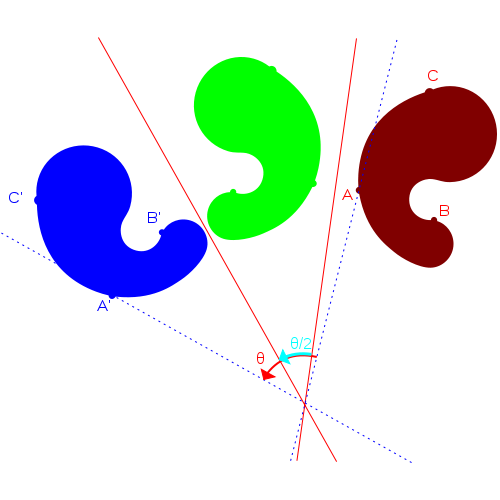
\includegraphics[scale=0.4]{rotation}
\caption{The product of two reflection matrices is a rotation matrix.}
\label{fig:rotation}
\end{figure}

\section{Positive Definite Matrices}

\chapter{Matrix Decomposition}
\section{LU Decomposition}
\section{QR Decomposition}
\section{Cholesky Decomposition}
\section{Symmetric Positive Definite (s.p.d.) Matrices}
\subsection{Cholesky Decomposition}
\deff{
	Let $\A$ be an $n \times n$ square matrix. $\A$ is said to be symmetric positive definite (s.p.d.) if
	\begin{align}
		\x^T \A \x > 0, ~~ \forall \x \ne \mathbf{0}
	\end{align}
}

\thm{\marginnote{\dbend}
	If $\A$ is s.p.d., then
	\begin{enumerate}
		\item The diagonal elements of an s.p.d. matrix are positive.
		\item All eigenvalues of $\A$ is positive.
		\item Its determinant is positive.
		\item It is nonsingular.
	\end{enumerate}
}
\noindent
\prof{
	The diagonal elements are positive because $a_{kk} = \e_k^T \A \e_k > 0$. The eigenvalues of an s.p.d. matrix are all positive is easy to prove by observing that $$0 < \x^T\A\x = \x^T\lambda\x = \lambda \|\x\|_2^2$$ The positivity of determinant can be shown by looking at the LDU decomposition. Finally, it is nonsingular because the determinant is nonzero.
}	
\deff{
	Let $\A$ be an $n \times n$ square matrix. A principal submatrix of $\A$ is obtained by selecting some rows and columns with the {\em{same}} index subset of $\{1, \cdots, n\}$.
}
\deff{
	Let $\A$ be an $n \times n$ square matrix. A {\em{leading}} principal submatrix of $\A$ is a principal submatrix of $\A$ with the index subset $\{1,\cdots,m\}$, for some $m \le n$.
}

\thm{\marginnote{\dbend}
	If $\A$ is s.p.d. then every principle submatrix is s.p.d..
}
\prof{
	Suppose $\A_p$ of size $p$ is a principle submatrix of $\A$. Since $\A$ is s.p.d., for any nonzero vector $\x$ we have $\x^T \A \x > 0$. Remove the corresponding coordinates of $\x$, same as those removed when creating the principle submatrix, and call it $\x_p$. Then the resulting vector $\x_p^T \A_p \x_p = \x^T \A \x > 0$.
}

\subsection{Cholesky Decomposition}
\deff{
	The Cholesky decomposition of an s.p.d. matrix $\A$ is of the form
	\begin{align}
		\A = \L\L^*
	\end{align}
	where $\L$ is a lower triangular matrix, with {\em{real and positive diagonal elements}}.
}

\section{Singular Value Decomposition (SVD)}

\section{Eigendecomposition}
\section{Jordan Decomposition}
\section{Schur Decomposition}